\subsection{Algoritmo de Shor}
La razones por las cuales el algoritmo de Shor es mas eficiente (ecuación \ref{eq:compledidad_cuantica}) que el algortimo de criba general del cuerpo de números (ecuación \ref{eq:O(clasico)}) son las siguientes:
\begin{itemize}
    \item Transformada de Fourier Cuántica.
    \item Periodo de la función a\textsuperscript{x}mod N.
\end{itemize}
\subsubsection{Transformada de Fourier Cuántica (QFT)}
La Transformada de Fourier Cuántica es una forma efectiva para realizar un cambio de base, este lo realiza de la base computacional $\lbrace \left|0 \right\rangle,\left|1 \right\rangle \rbrace$ hacia 
la base de Fourier $\lbrace \left| \tilde{0} \right\rangle,\left| \tilde{1} \right\rangle \rbrace$.
\begin{figure}[H]
    \begin{subfigure}{0.5\linewidth}
        \centering
        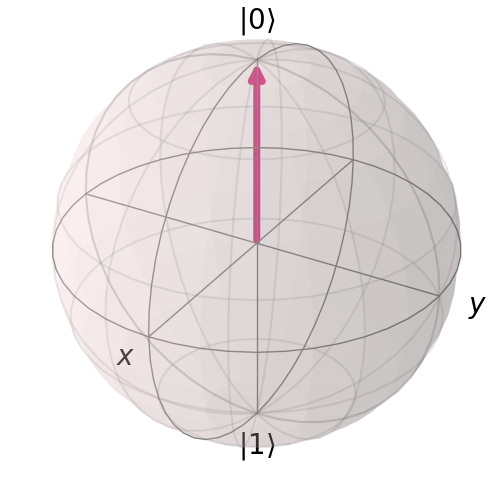
\includegraphics[scale=0.3]{images/0.png}
        \caption{Qubit con el estado cuántico $\left|0 \right\rangle$ representado en la esfera de Bloch.}
    \end{subfigure}
    \begin{subfigure}{0.5\linewidth}
        \centering
        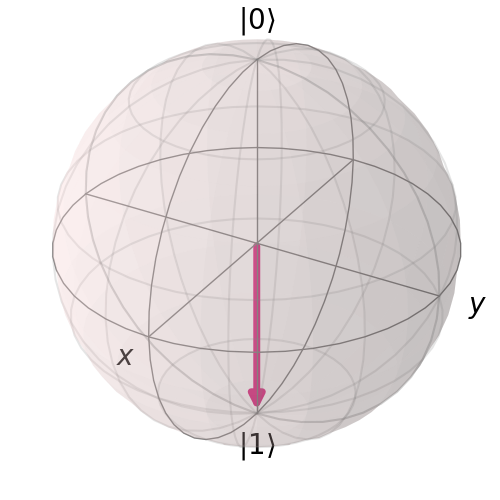
\includegraphics[scale=0.3]{images/1.png}
        \caption{Qubit con el estado cuántico $\left|1 \right\rangle$ representado en la esfera de Bloch.}
    \end{subfigure}
    \begin{subfigure}{0.5\linewidth}
        \centering
        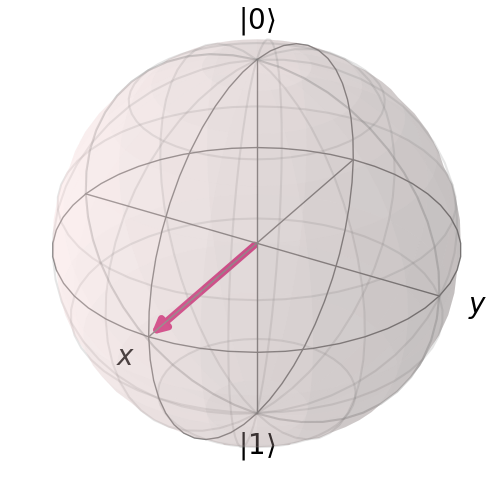
\includegraphics[scale=0.3]{images/2.png}
        \caption{Qubit con el estado cuántico $\left|\tilde{0} \right\rangle$ representado en la esfera de Bloch.}
    \end{subfigure}
    \begin{subfigure}{0.5\linewidth}
        \centering
        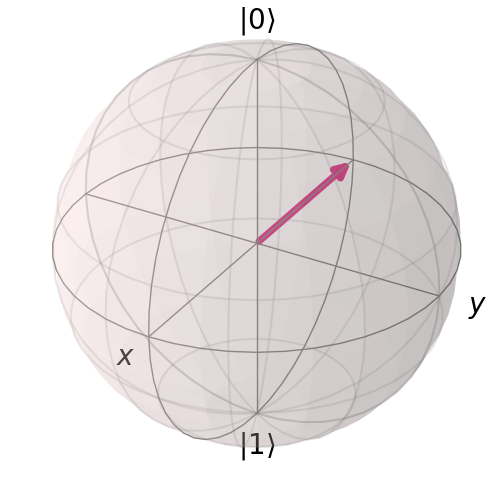
\includegraphics[scale=0.3]{images/3.png}
        \caption{Qubit con el estado cuántico $\left|\tilde{1} \right\rangle$ representado en la esfera de Bloch.}
    \end{subfigure}
\caption{Representación en la esfera de Bloch de los estados bases computacionales cuánticos y las bases de Fourier.}
\label{fig:QFT_bloch}
\end{figure}
Si se tienen n qubits, entonces existiran 2\textsuperscript{n} bases de estados. Definiendo a N como $N\equiv 2^n$, entonces:
\begin{align*}
    \left|\tilde{x} \right\rangle &\equiv QFT\left| x \right\rangle\\
    &= \frac{1}{\sqrt{N}} \sum\limits_{y=0}^{N-1} e^{\frac{2\pi i x y}{N}} \left|y \right\rangle
\end{align*}
Para el caso de un quibit, se tendria lo siguiente:\\
\begin{minipage}{0.5\linewidth}
    \begin{align*}
        \left|\tilde{0} \right\rangle &= \frac{1}{\sqrt{2}} \sum\limits_{y=0}^1 e^{\frac{2\pi i (0)y}{2}} \left|y \right\rangle \\
        &= \frac{1}{\sqrt{2}} \sum\limits_{y=0}^1 \left|y \right\rangle \\
        &= \frac{1}{\sqrt{2}} \left(\left| 0\right\rangle + \left| 1\right\rangle \right) \\
    \end{align*}  
\end{minipage}
\begin{minipage}{0.5\linewidth}
    \begin{align*}
        \left| \tilde{1} \right\rangle & = \frac{1}{\sqrt{2}} \sum\limits_{y=0}^1 e^{\frac{2\pi i (1)y}{2}} \left|y \right\rangle \\
        &= \frac{1}{\sqrt{2}} \left[e^{\frac{2\pi i(0)}{2}}\left| 0\right\rangle+ e^{\frac{2  \pi i 1}{2}} \left|1 \right\rangle\right] \\
        &= \frac{1}{\sqrt{2}} \left[\left|0 \right\rangle-\left|1 \right\rangle \right].\\
    \end{align*}
\end{minipage}
Con lo cual observamos que el estado $\left| 1\right\rangle$ al final queda multiplicado por un factor diferente a $1/\sqrt{2}$, extendiendo esta transformación para
k qubits, se tiene lo siguiente:
\begin{align*}
    \left|\tilde{x} \right\rangle &= \frac{1}{\sqrt{N}} \sum\limits_{y=0}^{N-1} e^{\frac{2\pi i xy}{N} }\left|y \right\rangle.\\
    &=\frac{1}{\sqrt{N}}  \sum\limits_{y_1=0}^1\sum\limits_{y_2=0}^1 \cdots \sum\limits_{y_k=0}^1 exp\left[\frac{2\pi i x}{N} \sum\limits_{k=1}^n y_k 2^{n-k}\right] \left| y_k \right\rangle.\\
    &= \frac{1}{\sqrt{N}} \sum\limits_{y_1,y_2,\cdots, y_k} \bigotimes\limits_{k=1}^n e^{\frac{2\pi i x}{N}y_k} \left| y_k \right\rangle.\\
    &=\frac{1}{\sqrt{N}} \bigotimes\limits_{k=1}^n \left[\left|0 \right\rangle+e^{\frac{2\pi i x}{N} 2^{n-k}} \left| 1\right\rangle  \right].\\
    &=\frac{1}{\sqrt{N}} \bigotimes\limits_{k=1}^N \left[\left|0 \right\rangle+e^{2\pi i x 2^{-k}} \left| 1\right\rangle  \right].\\
\end{align*}
Para obtener la transformada de Fouruier en base a los circuitos cuánticos, tenemos que realizar una serie de operaciones con la compuerta de Hadamard y la compuerta de rotaciones, en donde la 
fase de cada rotación es $exp(2\pi i / 2^k)$. La transformada de Fourier Cuática por si sola no nos ayuda en mucho, es por ello que se propuso un proceso en el cual
se pueda medir en que fase se encuentra el estado cuántico, esto lo lleva el proeso de estimación de fase cuántico (QPE).
\subsubsection{Estimación de Fase Cuántica (QPE).}

Al tener aplicada la transformada de Fourier Cuántica al estado de los qubits este contiene información en sus eigenvalores, ya que tienen la forma de
$e^{i\theta}$ y esto es que cada eigenvector forma una base ortonormal, es por ello que se tiene lo siguiente:
\begin{equation*}
    \mathcal{U} \left|\psi \right\rangle = e^{i\theta_\psi}\left|\psi \right\rangle.
\end{equation*}
Y el proposito de este proceso es obtener la fase $\theta_\psi$ dado del estado $\left|\psi \right\rangle$. Este mismo proceso se puede realizar usando 
el periodo de una función modular, la cual es $f(x)=a^xmodN$, la cual nos puede dar información acerca de la periodicidad de los residuos en una disivisón de valores.
\subsubsection{Periodo de la función a\textsuperscript{x}mod N}
Se tiene la función \begin{equation}
    f(x)=a^x mod N
    \label{eq:axmodn}
\end{equation}
donde $a$ y $N$ son enteros positivos tal que $a<N$ y que no tienen ningún factor en común. El periodo (o el orden r), es el valor más pequeño 
diferente de cero tal que:
\begin{equation}
    a^r mod N =1
    \label{eq:condicionr}
\end{equation}
Usando como ejemplos $a=3$ y $N=35$, se tiene el siguiente periodo:
\begin{figure}[H]
    \centering
    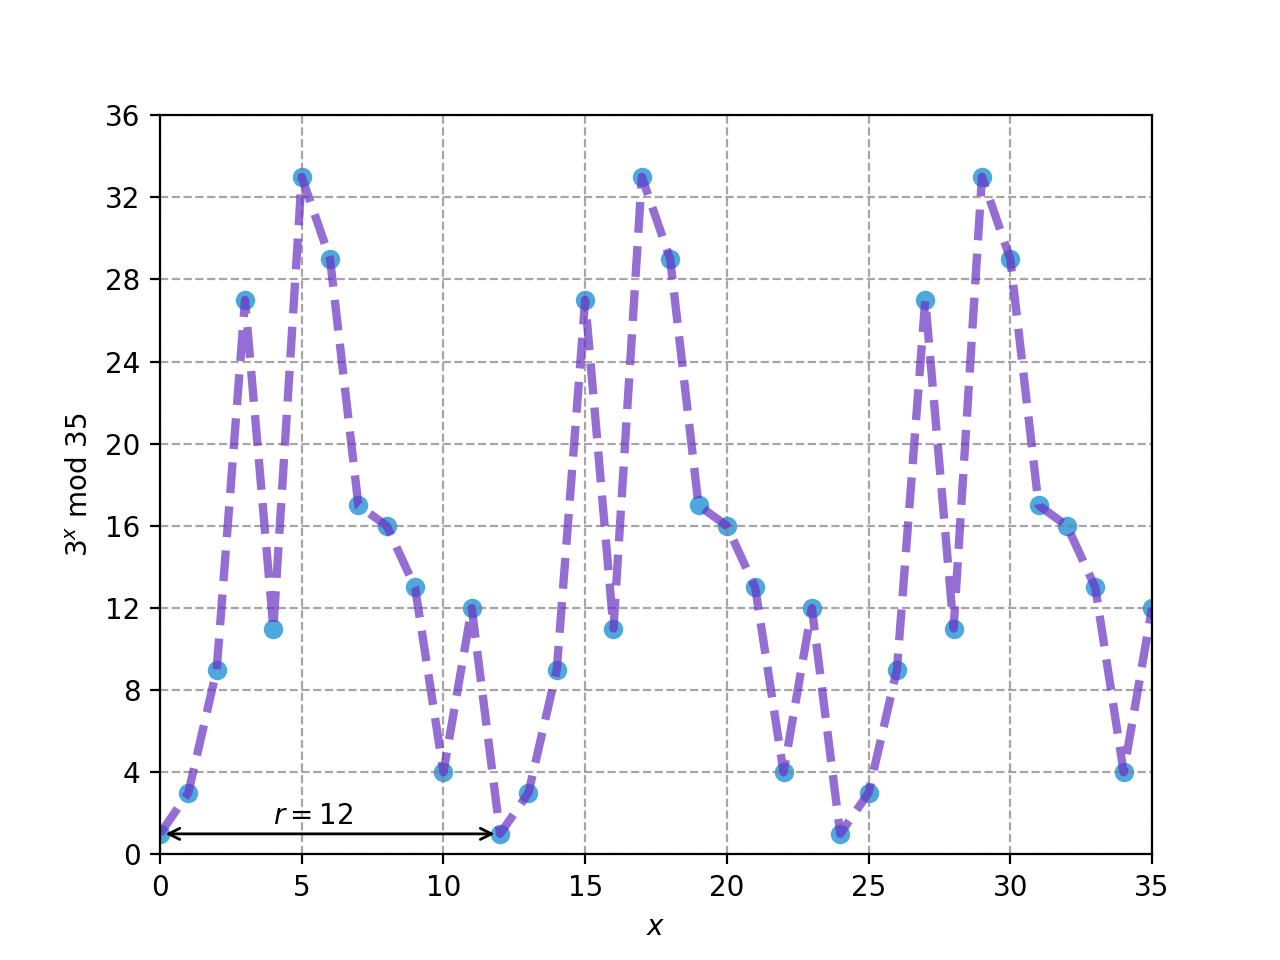
\includegraphics[scale=0.65]{../Graphics/period.png}
    \caption{Periodo de la función \ref{eq:axmodn} para visualizar la condición \ref{eq:condicionr} usando el código \ref{cod:rperiod}}
    \label{fig:condicionr}
\end{figure}
Para realizar esta operación dentro del Algoritmo de Shor se propusó un operador unitario tal que:
\begin{equation}
    U \left| y \right\rangle \equiv \left| ay mod N \right\rangle 
    \label{eq:umod}
\end{equation}
Para visualizar el funcionamiento de este operador se usará el ejemplo de $a=3$ y $N=35$, trabajando con los eigenestados de U empezando con el estado 
$\left|1\right\rangle$ podemos visualizar que la transformación sucesiva del operador U estariasmos multiplicando el estado por $amodN$, por lo tanto, después de
r transformaciones regresaremos al estado $\left|1\right\rangle$.
\begin{align*}
    U\left| 1 \right\rangle &= \left|3\right\rangle \\
    U^2\left| 1 \right\rangle &= \left|9\right\rangle \\
    U^3\left| 1 \right\rangle &= \left|12\right\rangle \\ 
                    & \vdots  \\ 
    U^{r-1}\left| 1 \right\rangle &= \left|12\right\rangle \\
    U^r\left| 1 \right\rangle &= \left|1\right\rangle \\
\end{align*}
Utilizando una superposición de estos estados, obtendremos lo siguiente:
\begin{equation}
    \left| u_0 \right\rangle = \frac{1}{\sqrt{r}} \sum\limits_{k=0}^{r-1} \left|a^k mod N \right\rangle.
    \label{eq:u0}
\end{equation}
Realizando esa serie para $a=3$ y $N=35$, encontramos que el estado descrito en \ref{eq:u0} es invariante bajo la transformación de U.
\begin{align*}
    \left| u_0 \right\rangle &= \frac{1}{\sqrt{12}} \left(\left|1\right\rangle + \left|3\right\rangle+ \left|9\right\rangle 
    +\cdots +\left|4\right\rangle + \left|12\right\rangle \right)\\
    U\left| u_0 \right\rangle &= \frac{1}{\sqrt{12}} \left(U\left|1\right\rangle + U\left|3\right\rangle+ U\left|9\right\rangle 
    +\cdots +U\left|4\right\rangle + U\left|12\right\rangle \right)\\
    &= \frac{1}{\sqrt{12}} \left(\left|3\right\rangle + \left|9\right\rangle+ \left|27\right\rangle 
    +\cdots +\left|12\right\rangle + \left|1\right\rangle \right)\\
    &= \left| u_0 \right\rangle .
\end{align*}
Lo cual obtenemos que el eigenvalor es 1. Un eigenestado más general es aquel el cual contenga una fase diferente para cada base de estados. Especificamente, veremos el caso
donde cada fase del k-esimo es proporcional a k, de tal manera que:
\begin{align}
    \label{eq:u1}
    \left| u_1 \right\rangle &= \frac{1}{\sqrt{r}} \sum\limits_{k=0}^{r-1} e^{-\frac{2\pi i k}{r}} \left| a^k mod N \right\rangle \\
    \label{eq:ua1}
    U\left| u_1 \right\rangle &= e^{\frac{2\pi i}{r}} \left| u_1 \right\rangle.
\end{align}
Teniendo así un único eigenestado para cada valor entero en $s$ donde $0\leq s \leq r-1$. Esto es muy conveniente, ya que realizando la suma de los eigenestados, las diferencias de fases
serán canceladas, obteniendo así el estado $ \left| 1 \right\rangle$.
\begin{equation*}
    \frac{1}{\sqrt{r}} \sum\limits_{s=0}^{r-1} \left|u_s \right\rangle =  \left| 1 \right\rangle.
\end{equation*}
Siendo así que el estado $ \left| 1 \right\rangle$ es una superposición de estos eigenestados, lo cual indica que podemos realizar 
el algoritmo de estimación de fase (QPE)  al operador U usando el estado $ \left| 1 \right\rangle$, para así obtener la medición de la fase:
\begin{equation*}
    \phi = \frac{s}{r}
\end{equation*}
Realizando del algoritmo de fracciones continuas sobre $\phi$ podemos encontrar el valor de ra. El circuito cuántico que realiza esta tarea es el siguiente:
\begin{figure}[H]
    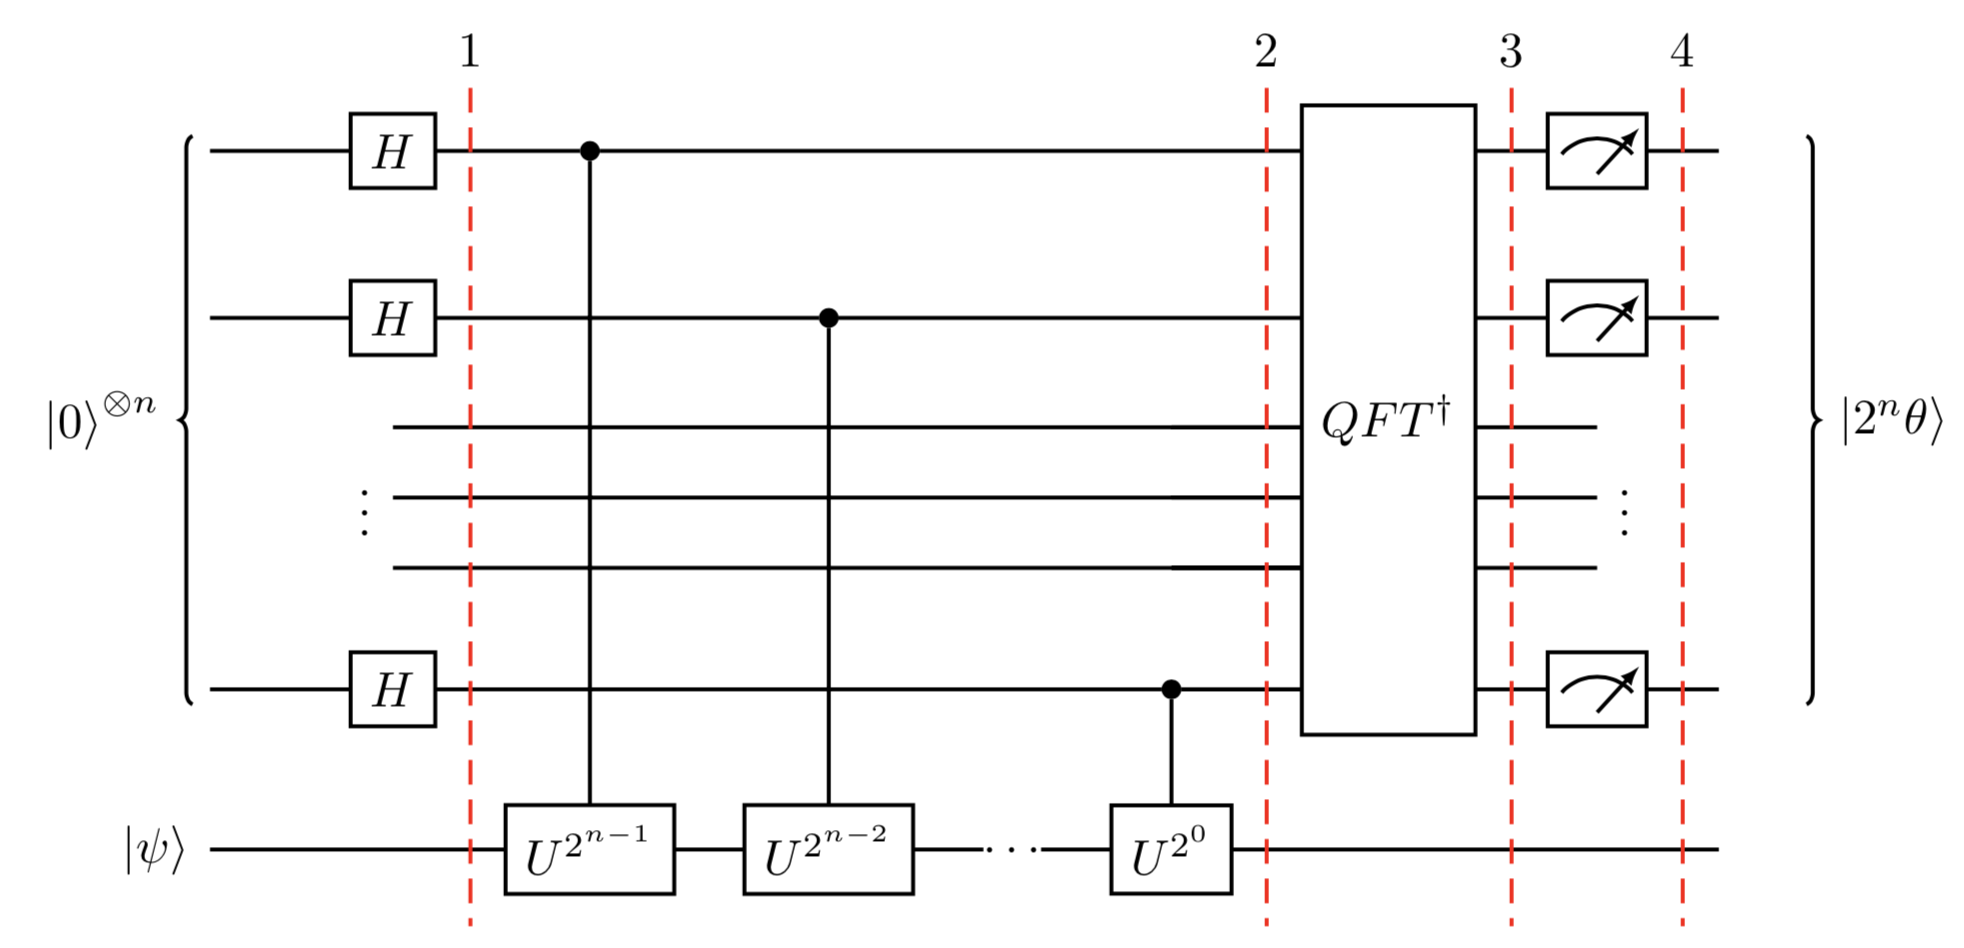
\includegraphics[scale=0.4]{../Graphics/qpe.png}
    \caption{Circuito cuántico que realiza el algortimo QPE (Quantum Phase Estimation) sobre una serie de qubits.}
    \label{fig:qpe}
\end{figure}
En la figura \ref{fig:qpe} se logra apreciar que existen varios pasos en el algoritmo los cuales son los siguientes:
\begin{enumerate}
    \item Los estados iniciales $\left|0  \right\rangle^{\bigotimes n}$ se les aplica la compuerta Hadamard a cada uno de ellos para lograr una superposición de ellos mismos.
    \item A cada estado se le aplica la compuerta de desplazamiento de fase para así obtener que se acerquen al estado en donde existe una periodicidad en la ecuación \ref{eq:condicionr}.
    \item Se aplica una transformada de Fourier inversa para obtener el estado cuántico después de haber sido rotados.
    \item Se realiza la medición de estos estados para obtener una estadistica y así llevar a conclusones acerca de las fases de los estados cuánticos.
\end{enumerate}